\section{Dependency Information}

No representation of trait ability mentioned so far specifically accounts for
dependency relationships between questions.  There are certainly dependency
relationships between whole (Bloom $\times$ concept) catogories.  For example,
one must be able to execute a for-loop (Comprehension of Loops) well before
gaining the ability to write one which satisfies an intended goal (Synthesis of
Loops). This is a course-grained dependency.

Other course-grained dependencies might be less obvious; questions in
categories for which concept is high-level and Bloom is low-level, depending on
questions in categories for which concept is lower-level and Bloom is
high-level.  For example, understanding a for-loop (Comprehension of Loops) is
predicated on being able to evaluate expressions (Application of Expressions).
In a trait ability matrix, these categories might even lie on a diagonal, which
would otherwise seem to suggest their independence.

Consider finer-grained dependency relationships among the following specific
questions regarding expressions:

\begin{verbatim}
 (a) What is (5 % 2)?
 (b) What is (5 / 2)?
 (c) What is (5 % (5 / 2))?
\end{verbatim}

The intuition captured by this example is that Part (c) could not be answered
correctly, at least not by any logical chain of reasoning, without possessing
the specific application ability that Part (a) and Part (b) test for.

It is probably true that Part (c) is more difficult than Part (a) or Part (b),
but this is not the reason for the dependency; rather it would appear the
dependency is the reason for the higher difficulty.  In terms of questions
which test application ability for expressions, all of the questions are in the
same neighborhood of difficulty; it is even possible albeit unlikely for the
$\beta$ values for all of these to be equal.  

However, if dependencies of the form $c \rightarrow a$ and $c \rightarrow b$
exist (that is, $c$ depends on $a$ and $b$), they may be indicated by a
high simple matching coefficient:

\begin{table}
 \caption{Notation for counts of joint observations}
 \vspace{12pt}
 \begin{tabularx}{\textwidth}{|X|X|X|X|}
 \hline
        & \y $y=0$         & \y $y=1$         & \y total     \\ \hline
  \y $x=0$ & $n_{00}$      & $n_{01}$      & $n_{0 \bullet }$  \\ \hline
  \y $x=1$ & $n_{10}$      & $n_{11}$      & $n_{1 \bullet }$  \\ \hline
  \y total & $n_{\bullet 0}$ & $n_{\bullet 1}$ & $n$                \\ \hline
 \end{tabularx}
\vspace{24pt}
\end{table}

\begin{equations}
  \frac{n_{00} + n_{11}}{n_{00} + n_{01} + n_{10} + n_{11}}
\end{equations}

where $n_{00}$ is the number of observations in which both questions are not
passed, $n_{01}$ and $n_{10}$ are the number of observations for which either
but not both questions are passed, and $n_{11}$ is the number of observations
for which both questions are passed.  This is assuming that the dependee is
scheduled prior to the depender question.  The notion expressed by a high
simple matching coefficient is that the depender is not passed if the dependee
is not passed; and the depender is passed if the dependee is passed.  

Alternatively, the phi coefficient, or mean square contingency coefficient,
can be used to identify the degree of association between two questions.
It is defined as:

\begin{equation}
 \phi = \frac{n_{11}n_{00} - n_{01}n_{10}}
 { 
   \sqrt{ n_{\bullet 0} n_{\bullet 1} n_{0 \bullet} n_{1 \bullet} } 
 }
\end{equation}

This is the binary analogue to the Pearson correlation coefficient; but its
range is only $[-1, 1]$ if there is a fifty-fifty split.  


\subsection{The Dependency Graph}

Items are organized into sets, called item sets.  Alternatively they may be
called assessments.  These are groups of items used for testing; practically
speaking, they may be tests, worksheets, homework assignments, and so forth. 

Subsets containing items which have dependency relationships form a directed
graph, specifically in form of a tree.  In such a tree graph, $x \rightarrow y$
indicates that $x$ depends on $y$.  In addition, as will be discussed later,
these edges have weights which indicate the extent of the dependency
relationship.  The root of each such tree is a depender.  Not all items in the
set are part of the same tree; there may thus be a forest for an item set.

\begin{figure}[!p]
\label{fig:forest}
  \centering\includegraphics{fig/forest.eps}
\caption{A forest obtained from an item set, where each tree is a subset
of the item set which has dependency relationships}
\end{figure}

\begin{figure}[!p]
\label{fig:severance}
  \centering\includegraphics{fig/severance.eps}
\caption{The severance of dependency relationships based upon low $\alpha$
values}
\end{figure}

There are two incarnations of each graph: one is a base dependency graph whose
nodes contain the item-specific information. The node $i$ for the ith item
contains item response theory parameters $\alpha_i$, $\beta_i$, and $\gamma_i$;
as well as a memorability parameter $\mu_i$, which is discussed in
Sec~\ref{sec:reactivation}.

The other is a student graph, which is a clone of the base dependency graph but
whose nodes contain the response information from the student.  The response
information is a list of 2-tuples containing the correctness of the response
and the timestamp of that response:

\begin{equations}
\label{eq:responses}
   \langle (x_1, t_1), (x_2, t_2), \ldots (x_n, t_n) \rangle
\end{equations}

An example of a base dependency graph is depicted in Fig~\ref{fig:base-graph};
and a student-specific dependency graph is depicted in
Fig~\ref{fig:student-graph}.

\begin{figure}[!p]
\label{fig:base-graph}
  \centering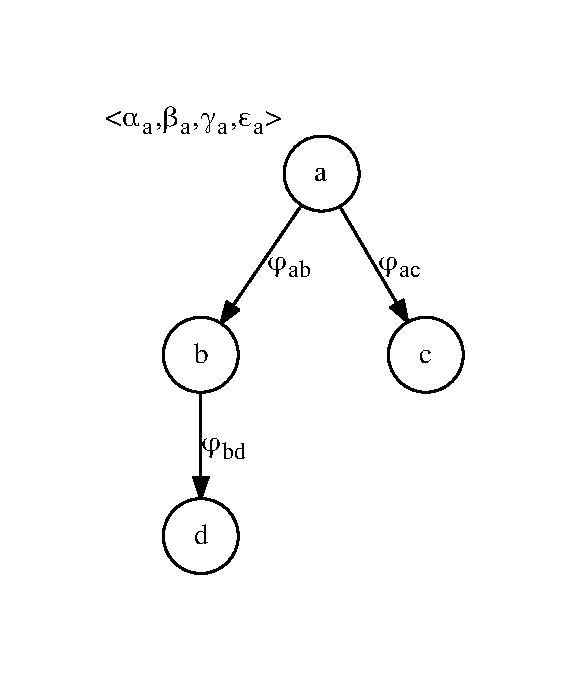
\includegraphics{fig/base-graph.eps}
\caption{The base item set graph, which includes item-specific paramters}
\end{figure}

\begin{figure}[!p]
\label{fig:student-graph}
  \centering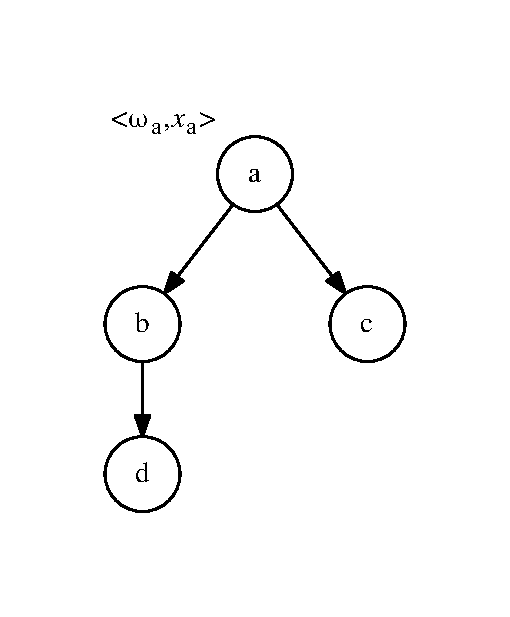
\includegraphics{fig/student-graph.eps}
\caption{The student-specific item set graph, which includes the list of
student responses and timestamps for each response}
\end{figure}

\subsection{Probability Estimates Using Dependees}

Logistic regression (pioneered by David Cox \cite{cox:1958}) is an ideal tool
for predicting success or failure given prior information about dependencies.
This is due to the fact that the dependent variable in question (the success of
answering a depender) is binary.  

One may wonder why any other form of regression technique is preferred over
linear regression.  Consider the linear equation in which a binary dependent
variable $Y$ depends on some response $X$:

\begin{equations}
         Y = a + bX + \epsilon
\end{equations}

where $a$ is some constant, $b$ is a coefficient, $\epsilon$ is the error, and
$Y$ assumes one of two possible values, 0 for failure or 1 for success.  Linear
regression has five assumptons, three of which are violated in this situation:

\begin{itemize}

  \item Linear relationship. Linear regressions require that linear
  relationships exist between the dependent variable and independent variables;
  however since the dependent variable assumes one of two possible values, the
  relationship is non-linear.

  \item Multivariate normality. This requirement holds that every linear
  combination of $k$ components has a univariate normal distribution.  This
  is not the case since each $k$ component assumes one of two possible values.

  \item Homoscedasticity. This requires that error terms along the regression
  are equal, but in the above situation, the variance of the error is dependent
  on the probability.   In particular $\mathrm{var}(\epsilon) = p(1-p)$.

\end{itemize} 

In addition, linear regressions require little to no multicollinearity; that
is, independent variables should be independent from one another; this may be
established by computing the correlation matrix for the independent variables.
Also, there should be no auto-correlation: $y_2$, the second observation,
should not depend on $y_1$.  This assumption is typically violated by time
series, but it is assumed to hold here because the dependent variables are
measured across students rather than time.  

Binary logistic regression assumes that:

\begin{itemize} 

 \item The dependent variable is binary,
 
 \item P(Y=1) is the probability that the event $Y$ occurs, 
 
 \item The model is fitted correctly, which means that there are no extraneous
 variables used in the regression, but that all variables are meaningful,

 \item That error terms should be independent; each observation should be
 independent, and little to no multicollinearity should exist.  

 \item Indepedent variables should be linearly related to the log odds of
 the event.

\end{itemize} 

It is important to note that the third assumption may or may not hold depending
on the correlations between the dependees.  The nature of the problem is such
that one expects dependee questions to be intercorrelated.  One possible remedy
is to group the questions to avoid intercorrelations.

Logistic regression is a regression of what are known as log odds. The odds
are defined as:

\begin{equations}
  \mathrm{odds} = \frac{p}{1-p}
\end{equations}

And the log odds, or logit, is defined as:

\begin{equations}
  \logit(y) = \ln(\mathrm{odds}) = \ln\Big(\frac{p}{1-p}\Big) = a + bX
\end{equations}

Correspondingly, odds may be defined as follows:

\begin{equations}
  \frac{p}{1-p} = e^{a + bx}
\end{equations}

Solving this equation for $p$ yields

\begin{equations}
  p = \frac{e^{a + bx}}{1 + e^{a + bx}}
\end{equations}

which can be reduced to 

\begin{equations}
  p = \frac{1}{1 + e^{-(a + bx)}}
\end{equations}

This is called the logistic curve, which is one in the family of sigmoid
curves.  It is identical to the type of curve used in Item Response Theory.
Compare the exponent in the Item Response Theory probability formula with 
the right-hand-side of the logit function:

\begin{equations}
  a + bx = \alpha(\beta - 1)\theta
\end{equations}

In the 2PL model, in which $\gamma_i$ is absent, the Item Response Theory
calculation of $\theta_s$ can be interpreted as a logistic regression in which
the unknown coefficient is $\theta_s$, the item-dependent inputs are given by
$\alpha(\beta-1)$, and the constant $a=0$.

Thus, a modified form of logistic regression may be sought.  It is desirable
to keep in account the item discrimination as well as the trait ability of
the student. 

\begin{equations}
  Y = b_1X_1 + b_2X_2 + \ldots + b_{n-1}X_{n-1} + b_n\alpha_i(\theta_s-\beta_i)
\end{equations}

In this expression, the term $\alpha_i(\theta_s-\beta_i)$ is retained, however
it is multiplied by a coefficient $b_n$ to determine its weight. Likewise
coefficients $b_1$, $b_2$, \ldots $b_{n-1}$ determine weights of the dependee
items.  This results in a probability function for answering the depender
question correctly given responses for the dependee questions:

\begin{equations}
  p = \frac{1}{1 + e^{b_1X_1 + b_2X_2 + \ldots + b_{n-1}X_{n-1} + b_n\alpha_i(\theta_s-\beta_i)}}
\end{equations}

To determine the individual contribution of each predictor (dependee), the
Wald statistic may be used.  It is defined as:

\begin{equations}
  W_i = \frac{b_i^2}{SE_{b_j}^2}
\end{equations}

If the statistic is sufficiently low, then the supposed dependee is likely not
a dependee at all, in which case the edge indicating the dependency
relationship may be pruned from the tree.  The logistic regression model will
naturally assign a low weight to such a dependee, and its use in the scheduling
algorithm will be limited by its relative weight.

\begin{figure}[!p]
\label{fig:neural}
  \centering\includegraphics[width=.6\textwidth]{fig/neural.eps}
\caption{A perceptron; a single-layer neural network, where the inputs a, b, and c
are multiplied by weights, summed, and applied to a sigmoid squash function}
\end{figure}

\begin{figure}[!p]
\label{fig:deps}
  \centering\includegraphics[width=.6\textwidth]{fig/deps.eps}
\caption{A view of the dependency graph and weights used in the logistic regression,
including the item parameters}
\end{figure}

The use of the logistic regression model in the intelligent tutoring system
suggests that the student would need to have answered all the dependencies
(that values of 0 or 1 are available).  In many instances where it is desirable
to use such a predictive model, this is not the case; instead what is available
is a probability that the student will be able to answer the question
correctly.  In such cases, the model is used with the probabilities calculated
using Item Response Theory.

The above probability estimates also assume an atemporal view of questions: if
the student has answered a question, the student remembers the answer to the
question permanently; however this is evidently not the case.  

What remains is a temporal account of questions, in particular the role of
memory and forgetting.


